\subsection{Steered Response Power}

Steered Response Power (SRP) source localization is a method to detect noise using beamforming techniques. SRP beamforms the signals and perform a cross correlation between the sensors to find the power of each beam. The computational demand rise very fast which makes it nearly impossible to implement in a real time applications, even if its performance in difficult condition outperform the TDOA based methods\cite{dmochowski2007generalized}. In this thesis, real time application is discarded so its application can be considered. The first part discuss the basic principles behind this method whereas the second part introduce an hybrid method that improve the computational time of SRP without decreasing its robustness. Sound localization using beamforming techniques was first introduced by Omologo and Svaizer in the 90`s \cite{omologo1997use} as "global coherence field", which used the level of correlation between two sensors to map a source location in space. While the generalized cross correlation is a simple cross correlation between each pair of microphone and only output an estimate of the time delay, the SRP method "beamform" the space and compute the energy of each location beam. The beam with the most energy is assumed to be the main sources in the case of free field propagation. In the same fashion as the GCC method proposed to prefilter the signal before performing the cross correlation for all the time delay, a PHAT can be applied on the beamformed signal, this method is called SRP-PHAT.

%\subsubsection{Steered Beamformer}

The SRP method is based on a regular delay-and-sum beamformer given by

\begin{equation}
    y_{\rho,\phi,\theta}(n)=\sum\limits_{m=0}^{M-1}{w_m x_m[n + f_{0,m}(\rho,\phi,\theta)]} 
\end{equation}

Where $f_{0,m}(\rho,\phi,\theta)$ is the relative delay from the reference sensor to the M sensor and $w_m$ the amplitude weight. When $w_m=1$, the output power of the beamformer is

\begin{equation}
    \mathbb{E}[{y_{\rho,\phi,\theta}(n)^2}]=\sum\limits_{i=0}^{M-1}\sum\limits_{j=0}^{M-1}{R_{x_i,x_j}[f_{i,j}(\rho,\phi,\theta)]} 
    \label{eq:poweroutputbeamformer}
\end{equation}

Usually cross correlation is computed in the frequency domain using cross-spectrum which is then inverse fast Fourier transformed (IFFT).

\begin{equation}
    R_{x_i,x_j}(\tau)= \sum\limits_{k=0}^{N_{f}-1}{X_{i}(k)X_{j}^*(k)e^{j2\pi\frac{k}{N_{f}}\tau}}
\end{equation}

%\subsubsection{SRP Search}

The SRP method starts with a look up procedure which associate each set of coordinate ($\rho,\phi,\theta$) to a given set of delays between each microphones. For instance, if we do not care about the range and use a 1 degree resolution, the SRP method associate 360*360=129600 positions to corresponding delays. The cross correlations at the particular delay are then computed. When the beamforming of the space and the computation of the cross correlation are completed the maximum value is chosen as the estimate of the main source in the case of single source detection. For multi sources, local maximas can also be selected. For a given position, the output of the SRP search is the sum of the cross correlation at each time delay found relative to each pair of microphone. It corresponds to the power output of the beamformer defined in equation \ref{eq:poweroutputbeamformer}
\begin{equation}
    S^{SRP}(\rho,\phi,\theta)=\sum\limits_{i=0}^{M-1}\sum\limits_{j=0}^{M-1}{R_{x_i,x_j}[f_{i,j}(\rho,\phi,\theta)]}
\end{equation}

The SRP method estimates the source location ($\Hat{\rho},\hat{\phi},\hat{\theta}$) after creating the SRP search space such that

\begin{equation}
    (\Hat{\rho},\hat{\phi},\hat{\theta})=\argmax_{\rho,\phi,\theta}S^{SRP}(\rho,\phi,\theta)
\end{equation}

%\subsubsection{Premapping the delays to potential sources locations}

The classical SRP search beamform sequentially the 3D space and locations [($\rho_{1},\phi_{1},\theta_{1}$), ($\rho_{2},\phi_{2},\theta_{2}$), ... ,($\rho_{x},\phi_{x},\theta_{x}$)] might be associated with the same relative delays $\tau_{1}$. The cross correlation at delay $\tau_{1}$ is then computed x times, which lead to the same results for each [($\rho_{1},\phi_{1},\theta_{1}$), ($\rho_{2},\phi_{2},\theta_{2}$), ... ,($\rho_{x},\phi_{x},\theta_{x}$)] positions, leading to numerous useless cross correlation computations. \cite{dmochowski2007generalized} propose an improvement on the SRP search algorithm by premapping the relative delays to their corresponding set of location. Instead of proceeding to a sequential search in the 3D space,a search on the relative possible delays is considered. The possible delays are known based on the array geometry and can be stored in memory. The cross correlations are calculated for each delay subset and related a set of potential source location in space in the final steps of the algorithm. Note that the computational cost gain is great for an array composed of a lot of microphones. In the case of 3 microphones, there is still a gain but it's definitely less than with 15 microphones. Also care should be taken if the array has a large aperture and is therefore subject to spatial aliasing. Prefiltering the signal before hand using PHAT introduce a function $\psi_{ij}$ in the cross correlation

\begin{equation}
    R_{x_i,x_j}(\tau)= \sum\limits_{k=0}^{N_{f}-1}{\psi_{ij} X_{i}(k)X_{j}^*(k)e^{j2\pi\frac{k}{N_{f}}\tau}}
\end{equation}
where
\begin{equation}
    \psi_{ij} = \frac{1}{|{X_{i}(k)X_{j}^*}|}
\end{equation}

\subsubsection{Hybrid SRP-PHAT}

\cite{peterson2005hybrid} describes a novel approach for sound localization using a two stage approach in order to reduce the computational load. The first stage identifies roughly the sources locations while the second stage is a modified version of the SRP-PHAT algorithm that only perform a grid search around the first stage estimated location. The method described in \cite{peterson2005hybrid} is well suited for near-field location using large aperture array which is not our requirement but the idea can be adapted in the case of far-field sound localization. Section \ref{sec:TDOA} gives an introduction to TDOA based localization and introduce the cone approximation for the far-field. The idea of the hybrid approach is to do a classical GCC-PHAT estimation to get the relative delays between the sensors. The delays estimate are use to derive the cone intersections which give a location estimate which is then inputed into a SRP-PHAT where the search region is constrained around the location estimates. A system overview of the algorithm is given in figure \ref{fig:hybridalgo}.

\begin{figure}[H]
    \centering
    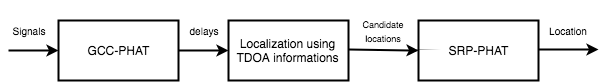
\includegraphics[width=1\textwidth]{Figures/hybridalgo.png}
    \caption{Simplified block diagram of the Hybrid algorthim}
    \label{fig:hybridalgo}
\end{figure}



